\documentclass[12pt, aspectratio=169]{beamer}

\usepackage[utf8]{inputenc} % кодировка
\usepackage[english, russian]{babel} % Система переносов
\usepackage[T2A]{fontenc} % font encoding

% \usepackage{tempora} % шрифт Tempora (Tempora-TLF)
\usepackage{paratype} % шрифт PT Serif Caption (PTSerifCaption-TLF)

% mathematical formulas
\usepackage{amssymb}
\usepackage{amsmath}
\usepackage{geometry}
\usepackage{amsfonts} % подкл. дополнительных мат. шрифтов
\usepackage{latexsym} % некоторые редкие символыs

\usepackage{animate}

\usetheme{Goettingen}

\title
{
    Равномерное распределение точек на сфере
}
\author
{
    И.Б.Рахимов \\
    Руководитель: О.Г.Корольков
}
\institute
{
    Воронежский Государственный Университет
}
\date
{
    \today
}
\titlegraphic
{
    
\includegraphics[width=2cm]{images/vsu_logo.jpg}
}

\begin{document}

%%%%%%%%%%%%%%%%%%%%%%%%%%%%%%
\begin{frame}[plain]
    \maketitle
\end{frame}
%%%%%%%%%%%%%%%%%%%%%%%%%%%%%%


%%%%%%%%%%%%%%%%%%%%%%%%%%%%%%
\section{Актуальность}

\begin{frame}
\frametitle{Актуальность}

\begin{itemize}
    \item Как можно более равномерное распределение точек на сфере — невероятно важная задача в математике, науке и компьютерных системах, а наложение сетки Фибоначчи на поверхность сферы при помощи равновеликой проекции — чрезвычайно быстрый и эффективный метод аппроксимации для её решения. В данной работе будет показано, как благодаря незначительным изменениям его можно сделать ещё лучше.

    \item Задача равномерного распределения точек на сфере имеет очень долгую историю. Это одна из самых хорошо исследованных задач в математической литературе по сферической геометрии. Она имеет критическую важность во многих областях математики, физики, химии, в том числе в вычислительных методах, теории приближений, теории кодирования, кристаллографии, электростатике, компьютерной графике, морфологии вирусов и многих других..
\end{itemize}

\end{frame}
%%%%%%%%%%%%%%%%%%%%%%%%%%%%%%


%%%%%%%%%%%%%%%%%%%%%%%%%%%%%%
\section{Цели и задачи}

\begin{frame}
\frametitle{Цели и задачи}

Цель:
\begin{itemize}
    \item Изучить и улучшить алгоритм распределения точек на сфере - наложение сетки Фибоначчи.
\end{itemize}

Задачи:
\begin{itemize}
    \item Изучение совеременных подходов к решению задачи распределения точек на сфере;
    \item Изучения алгоритма наложения сетки Фибоначчи;
    \item Улучшение алгоритма наложения сетки Фибоначчи;
    \item Анализ разработанного алгоритма;
    \item Программная реализация алгоритма наложения сетки Фибоначчи.
\end{itemize}

\end{frame}
%%%%%%%%%%%%%%%%%%%%%%%%%%%%%%


%%%%%%%%%%%%%%%%%%%%%%%%%%%%%%
\section{Оптимизация расстояния упаковки}

\begin{frame}
\frametitle{Оптимизация расстояния упаковки}

 Часто эту задачу называют задачей Тэммса в честь ботаника Тэммса, искавшего объяснение структуры поверхности пыльцевых зёрен. Критерий упаковки требует от нас максимизировать наименьшее расстояние между соседями для $N$ точек. То есть

\begin{displaymath}
    d_N = \min_{i \neq j} \Vert x_i - x_j \Vert _2,
\end{displaymath}
  
\end{frame}

%%%%%%%%%%%%%%%

\begin{frame}
\frametitle{Оптимизация расстояния упаковки}

Аналогичным образом эти множества точек можно перенести из единичного квадрата $[0, 1]^2$ на сферу при помощи цилиндрической равновеликой проекции:

\begin{displaymath}
    (x,y) \rightarrow (\theta, \phi) : \quad \left( \cos^{-1}(2x-1) - \frac{\pi}{2}, 2\pi y \right),
\end{displaymath}

\begin{displaymath}
    (\theta,\phi) \rightarrow (x,y,z) : \quad \left (\cos\theta \cos\phi, \cos \theta \sin \phi, \sin \theta \right).
\end{displaymath}
  
\end{frame}

%%%%%%%%%%%%%%%%%%%%%%%%%%%%%%


%%%%%%%%%%%%%%%%%%%%%%%%%%%%%%
\section{Сетка Фибоначчи}

\begin{frame}
    \frametitle{Сетка Фибоначчи}
    \begin{columns}
        \begin{column}{0.5\textwidth}
            \begin{center}
                \begin{tabular}{ c } 
                    \animategraphics[autoplay, loop, width=3cm]{1}{animation/1/}{1}{3} \\
                    \animategraphics[autoplay, loop, width=3cm]{1}{animation/2/}{1}{3} \\
                \end{tabular}
            \end{center}
        \end{column}

        \begin{column}{0.5\textwidth}
            \begin{figure}[h!]
                \centering{Одно очень элегантное решение моделирует узлы, встречающиеся в природе, например, распределение семян в подсолнухе или сосновой шишке. Это явление называется спиральным филлотаксисом. Коксетер показал, что такие структуры имеют фундаментальную связь с рядом Фибоначчи}
            \end{figure}
        \end{column}
    \end{columns}  
\end{frame}
%%%%%%%%%%%%%%%%%%%%%%%%%%%%%%


%%%%%%%%%%%%%%%%%%%%%%%%%%%%%%
\section{Анализ $d_N^*$ при разных $\epsilon$}

\begin{frame}
  \frametitle{Анализ $d_N^*$ при разных $\epsilon$}
  \begin{columns}
    \begin{column}{0.5\textwidth}
      \begin{figure}[h!]
        Различные значения $d_N^*$ при разных значениях $\epsilon$. Чем больше значение, тем оптимальнее конфигурации. Мы видим, что $\epsilon \simeq 2.5$ обеспечивает решение, близкое к оптимальному.
      \end{figure}
    \end{column}
    \begin{column}{0.5\textwidth}
      \begin{figure}[h!]
        \centering{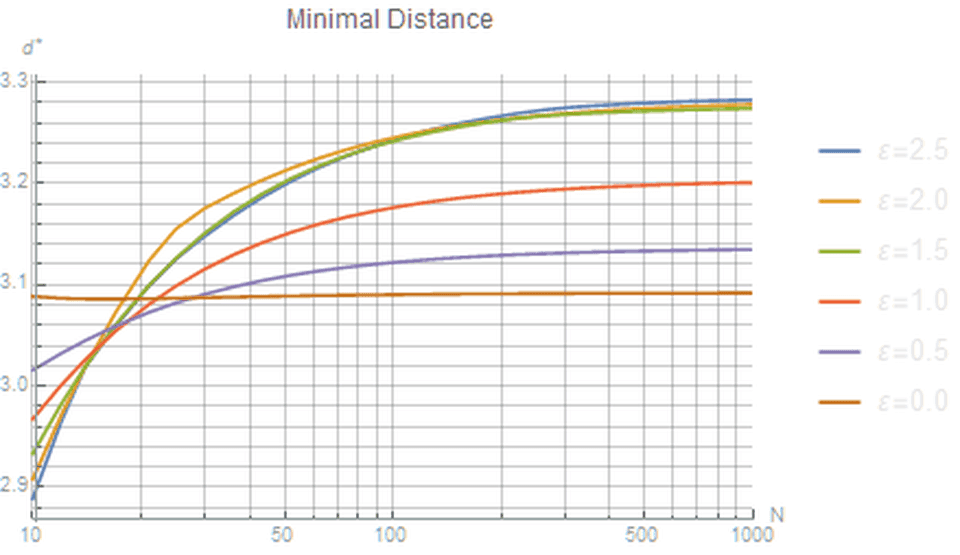
\includegraphics[scale=0.2]{images/2.png}}
      \end{figure}
    \end{column}
  \end{columns}  
\end{frame}
%%%%%%%%%%%%%%%%%%%%%%%%%%%%%%


%%%%%%%%%%%%%%%%%%%%%%%%%%%%%%
\section{Выводы}

\begin{frame}
\frametitle{Выводы}

\begin{itemize}
    \item Изучен и улучшен алгоритм распределения точек на сфере - наложение сетки Фибоначчи.
    \item Изучены совеременные подходовы к решению задачи распределения точек на сфере;
    \item Изучен алгоритм наложения сетки Фибоначчи;
    \item Улучшен алгоритм наложения сетки Фибоначчи;
    \item Проведён анализ разработанного алгоритма;
    \item Алгоритм был программно реализован.
\end{itemize}
  
\end{frame}
%%%%%%%%%%%%%%%%%%%%%%%%%%%%%%


%%%%%%%%%%%%%%%%%%%%%%%%%%%%%%
\section{Направления дальнейшей работы}

\begin{frame}
\frametitle{Направления дальнейшей работы}

\begin{itemize}
\item Адаптировать данный алгоритм для естественного распределения объектов (деревьев, волос и т.д.) на геометрии
\end{itemize}
  
\end{frame}
%%%%%%%%%%%%%%%%%%%%%%%%%%%%%%


%%%%%%%%%%%%%%%%%%%%%%%%%%%%%%
\author
{
    И.Б.Рахимов \\
    Руководитель: О.Г.Корольков \\
    Спасибо за внимание
}
\begin{frame}[plain]
    \maketitle
\end{frame}
%%%%%%%%%%%%%%%%%%%%%%%%%%%%%%

\end{document}